\chapter{\LaTeX{} Examples}
This section contains \LaTeX{} examples.  \warning{Remove it before printing the final version.}

The source code for these examples is in the \textit{LaTeX Examples.tex} file.  Its inclusion into the final document is controlled in the \textit{Model Comparison Report.tex} file.

% CITATIONS
\section{Citations}
% Citation example.
%DY: uncomment
This is a citation example \textcode{\tbs{}referencename\~\tbs{}cite\{ref:aarsnes2017a\}}.
\referencename~\cite{ref:aarsnes2017a}

% Add to bibliography without directly citing.
You can add a reference to the bibliography without directly citing it in text by using the command \textcode{\tbs{}nocite}, e.g., \textcode{\tbs{}nocite\{ref:abbassian1998a\}}.
% \nocite{ref:abbassian1998a}

\section{Built in Name Commands}
\begin{bulletedlist}
	\item \appendixname{} (\textcode{\tbs{}appendixname})
	\item \chaptername{} (\textcode{\tbs{}chaptername})
	\item \equationname{} (\textcode{\tbs{}equationname})
	\item \figurename{} (\textcode{\tbs{}figurename})
	\item \referencename{} (\textcode{\tbs{}referencename})
	\item \sectionname{} (\textcode{\tbs{}sectionname})
	\item \tablename{} (\textcode{\tbs{}tablename})
\end{bulletedlist}

% FIGURES
\section{Figures}
The \figurename~\ref{fig:lelatexlogo} shows the CNPC logo.  Note, don't add the end of sentence period for the short title in the caption (part between the []).
\begin{figure}
	\centering
	
\includegraphics[height=0.85in]{lelatexlogo}
	\caption[Short title for list of figures]{Longer title.  This is descriptive and can be multiple sentences.}
	\label{fig:lelatexlogo}
\end{figure}
\begin{figure}
	\centering
	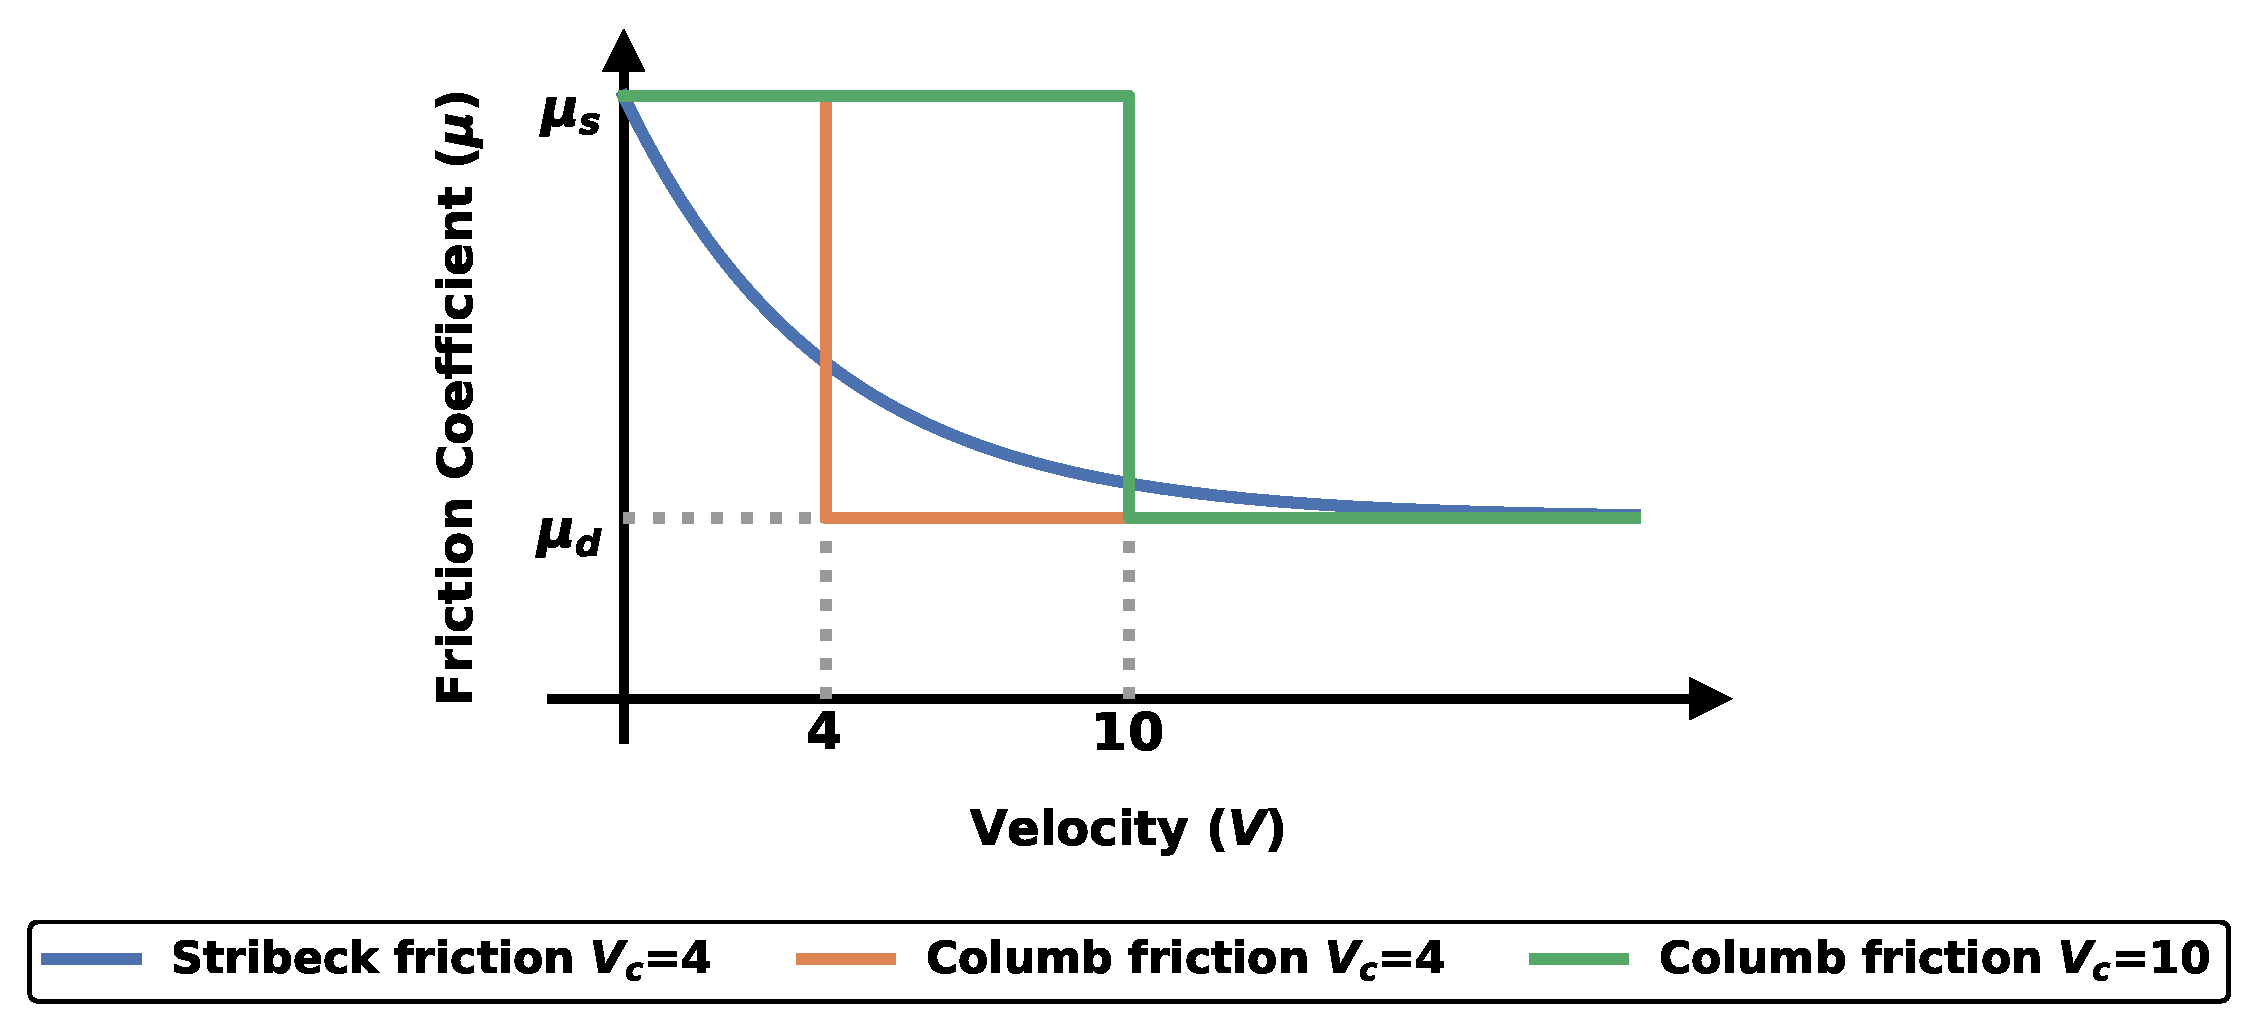
\includegraphics[height=2.5in]{exampleepsfigure}
	\caption[EPS example]{An example EPS image used as a figure.}
	\label{fig:exampleepsfigure}
\end{figure}

% LISTS
\section{Lists}
\begin{bulletedlist}
	\item The first bullet point.
	\begin{bulletedlist}
		\item Lists can include other lists.
		\begin{plainlist}
			\item A list with no markers.
		\end{plainlist}
	\end{bulletedlist}
	\item The second bullet point.
	\begin{numberedlist}
		\item Item 1.
		\item Item 2.
	\end{numberedlist}
\end{bulletedlist}


\section{MATH}
The (fake) calculation can be done using \equationname~\ref{eq:example}
\begin{equation}
	\alpha = 2\beta\sum \left( \frac{\gamma}{\sigma} \right)
	\label{eq:example}
\end{equation}
\begin{mathwhere}[0.3in] % <= The distance in the square brackets ([]) changes the space between the item being defined and the equal sign.
	\mathdefitem{\alpha}{the first variable;}
	\mathdefitem{\beta}{the second variable;}
	\mathdefitem{\gamma}{the third variable;}
	\mathdefitem{\sigma}{the final variable.}
\end{mathwhere}
This example demonstrates specially written \textcode{mathwhere} environment define the variables.  The \textcode{mathwhere} environment uses an optional argument to specify where the equal sign is placed.  See the source code for more information.  The environment takes the form of
\begin{plainlist}
	\item \textcode{\tbs{}begin\{mathwhere\}[distance]}
	\begin{plainlist}
		\item \textcode{\tbs{}mathdefitem\{math\}\{definition\}}
	\end{plainlist}
	\item \textcode{\tbs{}end\{mathwhere\}}
\end{plainlist}
\begin{mathwhere}[0.85in]
	\mathdefitem{\textrm{distance}}{the space allowed for the item being defined (location of the equal sign);}
	\mathdefitem{\textrm{math}}{a variable to define;}
	\mathdefitem{\textrm{definition}}{the definition of the variable.}
\end{mathwhere}


\section{Code}
\begin{code}{}
    \codeitem \codepragma{} \codemessage{}("// TO DO") \\
    \stepcodelevel
        \codenew{} Triangle();\\
        \prevcodelevel
\end{code}


% SPECIAL COMMANDS
\section{Special Commands}
Leave a note to finish a section later.
\notfinished{}

\editorsnote{This is a note.}

Other commands include the following.
\begin{bulletedlist}
	\item \important{important}
	\item \warning{warning}
	\item \note{Does not print this.} \tbs{}note\{...\} (doesn't print the argument)
\end{bulletedlist} 